\section{Поступательное движение твёрдого тела}

Под \textit{поступательным} движением абсолютно твёрдого тела понимают такое его
движение, при котором прямая, проведённая через любые две точки тела и жёстко с
ним связанная, остаётся во всё время движения \textit{параллельной самой себе}.

Точки \textit{поступательно} движущегося тела могут описывать \textit{любые
криволинейные траектории}, но движение тела сохраняет свой
\textit{поступательный} характер.

\begin{theorem}
  При поступательном движении твёрдого тела все его точки описывают одинаковые
  траектории и в любой момент времени имеют одинаковые скорости и ускорения.
\end{theorem}

\begin{figure}[H]
  \centering
  \resizebox{\linewidth}{!}{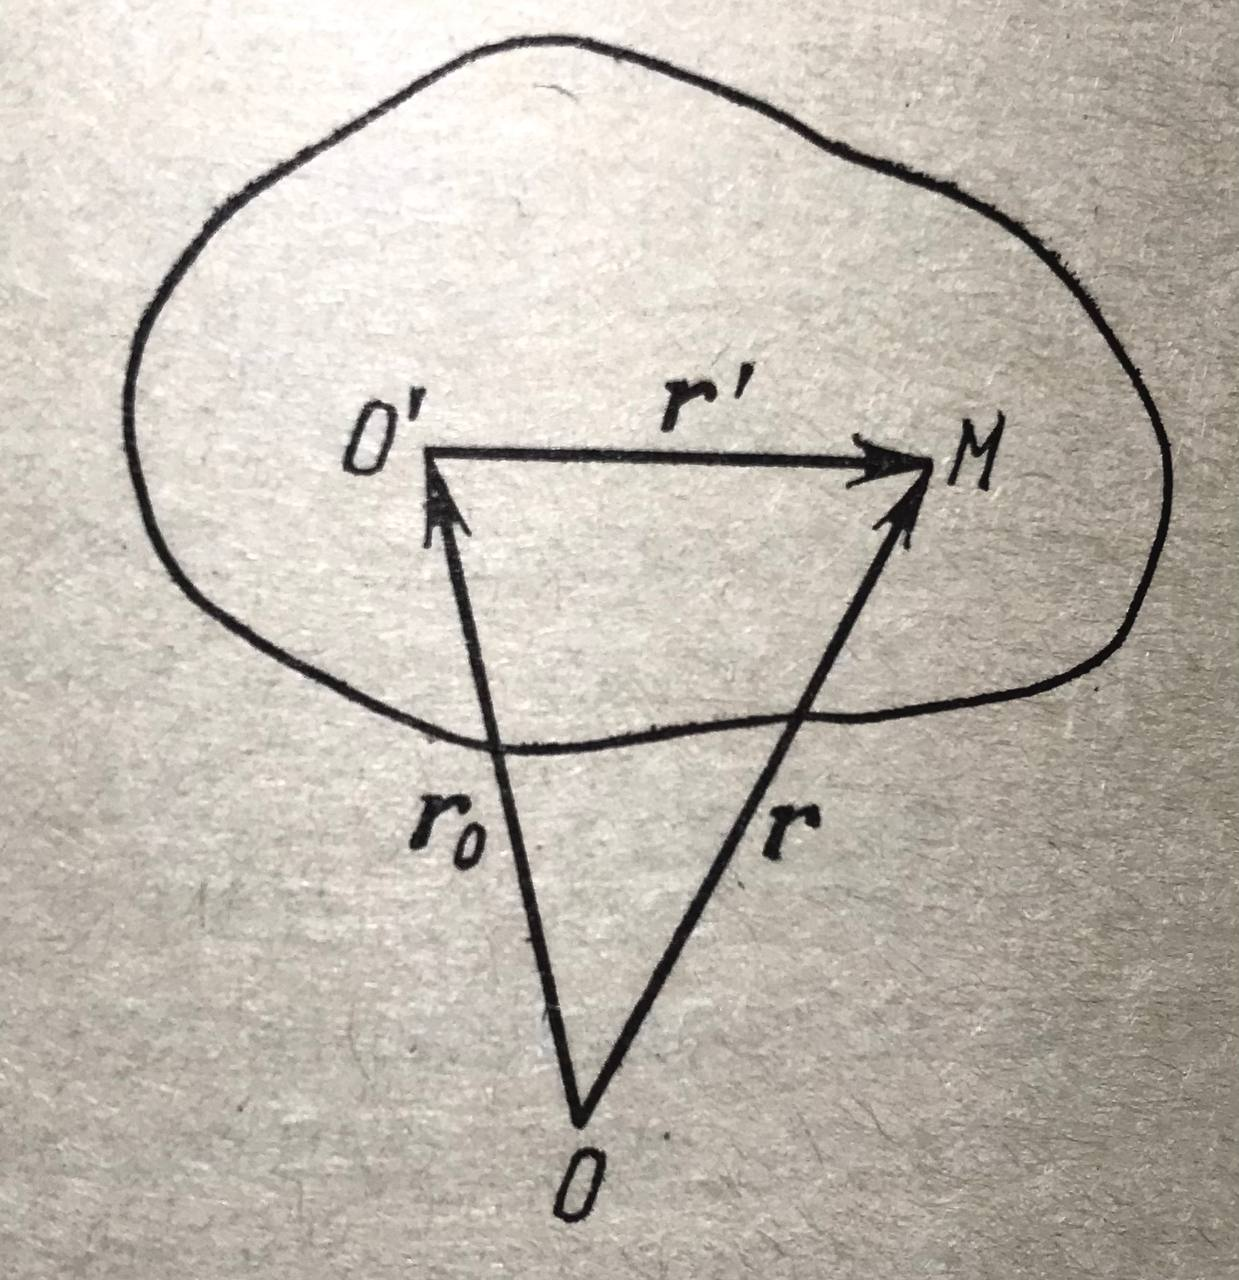
\includegraphics{src/mechanics/pictures/12_1.jpg}}

  \caption{}
  \label{fig:trajectory_carryover}
\end{figure}

\begin{proof}
  Определим положение любой точки $M$ твёрдого тела вектор-радиусом $\pvec{r}$,
  проведённым из некоторой точки $O'$, также принадлежащей телу. Если движение
  поступательное, то по определению вектор $\pvec{r}$ остаётся параллельным
  самому себе. Величина вектора $\pvec{r}$ ($r' = O'M$) не изменяется, так как
  тело твёрдое. Итак, $\pvec{r}$ является постоянным вектором.

  Обозначим через $\vec{r}_0$ вектор-радиус точки $O'$ относительно некоторой
  неподвижной точки $O$. Равенство
  \begin{equation}
    \label{eq:trajectory_translational}
    \vec{r} = \vec{r}_0 + \pvec{r}
  \end{equation}
  показывает, что траектория точки $M$ получается из траектории точки $O'$ путём
  параллельного перенесения её на постоянный по величине и направлению вектор.
  Следовательно, \textit{траектории точек твёрдого тела, движущегося
  поступательно, представляют собой конгруэнтные кривые}, получающиеся друг из
  друга путём параллельного переноса.

  Дифференцируя обе части формулы \ref{eq:trajectory_translational} по времени и
  замечая, что производная постоянного вектора $\pvec{r}$ равна нулю, получим
  \begin{equation*}
    \dt[\vec{r}] = \dt[\vec{r}_0],
  \end{equation*}
  или, вспоминая определение вектора скорости,
  \begin{equation}
    \label{eq:velocity_translational}
    \vec{v} = \vec{v}_0,
  \end{equation}
  то есть \textit{скорости всех точек твёрдого тела, движущегося поступательно,
  в любой момент времени друг другу равны как по величине, так и по
  направлению}.

  Дифференцируя обе части \ref{eq:velocity_translational} ещё раз по времени,
  получаем
  \begin{equation}
    \label{eq:acceleration_translational}
    \vec{w} = \vec{w}_0,
  \end{equation}
  то есть \textit{ускорения всех точек поступательно движущегося твёрдого тела в
  любой момент времени одинаковы}.
\end{proof}

\subsection{Список литературы}
\begin{enumerate}
  \item \cite{lourie}
\end{enumerate}

